%tikz绘图
%用axis画出一个平面直角坐标系
%定义变量MAX,取值6
%坐标系:domain:-MAS~MAX
%画出网格线,颜色black!10
%xtick和ytick的增量为2
%增加一个函数图象y=-x,x \in [-MAX+1,MAX-1]
%在第二象限的函数图象旁边标注y=-x

\documentclass[tikz,border=10pt]{standalone}
\usepackage{pgfplots}
\pgfplotsset{compat=1.18}
\begin{document}

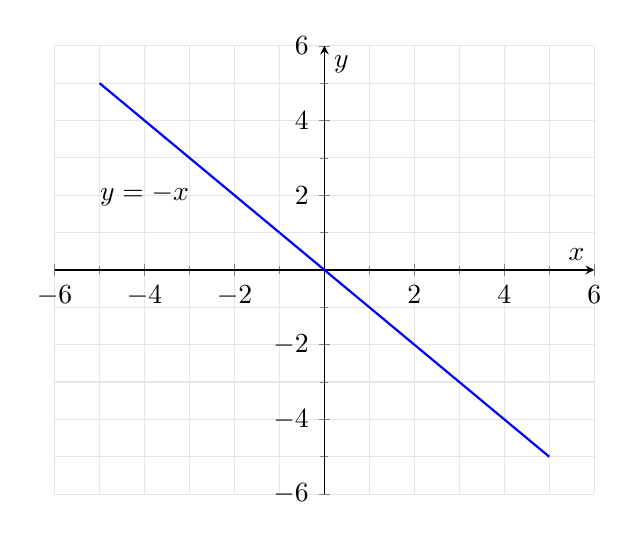
\begin{tikzpicture}
    \def\MAX{6} % 定义 MAX 变量,值为 6
    \begin{axis}[
        axis lines = middle,
        xlabel = {$x$},
        ylabel = {$y$},
        xmin = -\MAX, xmax = \MAX,
        ymin = -\MAX, ymax = \MAX,
        grid = both,
        minor tick num = 1,
        major tick length = 0.15cm,
        grid style = {black!10},
        xtick = {-6, -4, -2, 0, 2, 4, 6},
        ytick = {-6, -4, -2, 0, 2, 4, 6},
        domain = -\MAX:\MAX,
    ]
    % 绘制函数y=-x
    \addplot[blue, domain=-\MAX+1:\MAX-1, samples=100, thick] {(-x)};
    % 在第二象限的函数图象旁边添加标注
    \node at (-4,2) {$y=-x$}; % 标注在第二象限
    \end{axis}
\end{tikzpicture}

\end{document}
